\chapter{Решение задачи декодирования в пространстве высокой размерности}
\label{chap:ch2}

\section{Формальная постановка задачи}

Для постановки задачи декодирования введём предположения о структурах пространств $\bbX$ и $\bbY$.
\begin{assumption}
	Рассмотрим случай, когда пространства $\bbX$ и $\bbY$ избыточны. Это означает, что объекты $\bx$ и $\by$ живут на некоторых многообразиях низкой размерности. В простейшем случае такие многообразия могут являться линейными подпространствами.
\end{assumption}

\begin{definition}
	Назовём пространство $\bbT \subset \bbR^l$ \textit{скрытым пространством} для пространства $\bbX \in \bbR^n$ ($l \leq n$), если существуют функция $\varphi_e: \bbX \to \bbT$ и функция $\varphi_d: \bbT  \to \bbX$ такие что
	\[
	\forall \bx \in \bbX \quad \exists \bt \in \bbT: \varphi_d (\varphi_e(\bx)) = \varphi_d(\bt) = \bx.
	\]
	Функцию $\varphi_e(\bx)$ будем называть \textit{функцией кодирования} объекта $\bx$, функцию $\varphi_d(\bt)$ будем называть \textit{функцией декодирования}. 
	
	
	Аналогично введём определение \textit{скрытого пространства}~$\bbU \subset \bbR^s$ для целевого пространства $\bbY$, \textit{функции кодирования} $\psi_e: \bbY \to \bbU$ и \textit{декодирования} $\psi_d: \bbU  \to \bbY$
	\[
	\forall \by \in \bbY \quad  \exists \bu \in \bbU: \psi_d (\psi_e(\by)) = \psi_d(\bu) = \by.
	\]
\end{definition}

\begin{definition}
	Будем считать, что пространство $\bbT \subset \bbR^l$ задаёт \textit{внутреннюю структуру} пространства $\bbX \in \bbR^n$, если пространство $\bbT$ является скрытым для пространства $\bbX$.
\end{definition}

\begin{definition}
	Между пространствами $\bbX$ и $\bbY$ существует \textit{согласующее отображение}, если существуют пространства $\bbT$ и $\bbU$, задающие внутренние структуры для пространств $\bbX$ и $\bbY$ соответственно, и существует \textit{функция согласования} $g: \bbT \rightarrow \bbU$, такая что
	\[
	\forall \bu \in \bbU \quad \exists \bt:  \bu = g(\bt).
	\]
\end{definition}

\begin{assumption}
	Предположим, что в задаче предсказания~\eqref{ch1:eq:loss_min} пространства $\bbT$ и $\bbU$ задают внутреннюю структуру пространств $\bbX$ и $\bbY$. 
	Предположим также, что для данных скрытых пространств $\bbT$ и $\bbU$ существует функция согласования~$g: \bbT \rightarrow \bbU$. Тогда выполнено
	\[
	\forall \by \in \bbY \quad \exists \bx \in \bbX: \by = \psi_d(\bu) = \psi_d(g(\bt)) = \psi_d(g(\phi_e(\bx))). 
	\]
	
	Тогда общая схема задачи декодирования принимает вид следующей коммутативной диаграммы:
	\begin{equation}
		\begin{tikzpicture}
			\matrix (m) [matrix of math nodes,row sep=3em,column sep=4em,minimum width=2em]
			{
				\bbX \subset \bbR^n & \bbY \subset \bbR^r \\
				\bbT \subset \bbR^l & \bbU \subset \bbR^s \\};
			\path[-stealth]
			(m-1-1) edge node [above] {$f$} (m-1-2)
			(m-2-1) edge [bend right=10] node [right] {$\varphi_d$} (m-1-1)
			(m-2-2) edge [bend left=10] node [left] {$\psi_d$} (m-1-2)
			(m-1-1) edge [bend right=10] node [left] {$\varphi_e$} (m-2-1)
			(m-1-2) edge [bend left=10] node [right] {$\psi_e$} (m-2-2)
			(m-2-1) edge node [above] {$h$} (m-2-2);
		\end{tikzpicture}
		\label{ch1:eq:decoding_scheme}
	\end{equation}
\end{assumption}

\begin{definition}
	Согласно схеме~\eqref{ch1:eq:decoding_scheme}, определим модель декодирования $f: \bbX \rightarrow \bbY$ как суперпозицию
	\begin{equation}
		f = \psi_d \circ g \circ \varphi_e.
		\label{ch1:eq:def_decoding_function}
	\end{equation}
\end{definition}

\section{Доказательство корректности работы алгоритмов PLS и CCA}

Псевдокод метода регрессии PLS приведен в алгоритме~\ref{ch1:pls_pseudocode}.
Алгоритм итеративно на каждом из $l$ шагов вычисляет по одному столбцу $\bt_k$, $\bu_k$, $\bp_k$, $\bq_k$ матриц $\bT$, $\bU$, $\bP$, $\bQ$ соответственно. 
После вычисления следующего набора векторов из матриц $\bX$, $\bY$ вычитаются очередные одноранговые аппроксимации. 
При этом предполагается, что исходные матрицы~$\bX$ и~$\bY$ нормированы (имеют нулевое среднее и единичное среднее отклонение).

\begin{algorithm}[h]
	\caption{Алгоритм PLS}
	\label{ch1:pls_pseudocode}
	\begin{algorithmic}[1]
		\REQUIRE $\bX, \bY, l$;
		\ENSURE $\bT, \bP, \bQ$;
		\STATE нормировать матрицы $\bX$ и $\bY$ по столбцам
		\STATE инициализировать $\bu_0$ (первый столбец матрицы $\bY$)
		\STATE $\bX_1 = \bX; \bY_1 = \bY$
		\FOR{$k=1,\dots, l$}
		\REPEAT
		\vspace{0.1cm}
		\STATE $\bw_k := \bX_k^{\T} \bu_{k-1} / (\bu_{k-1}^{\T} \bu_{k-1}); \quad \bw_k: = \frac{\bw_k}{\| \bw_k \|}$
		\vspace{0.1cm}
		\STATE $\bt_k := \bX_k \bw_k$
		\vspace{0.1cm}
		\STATE $\bc_k := \bY_k^{\T} \bt_k / (\bt_k^{\T} \bt_k); \quad \bc_k: = \frac{\bc_k}{\| \bc_k \|}$
		\vspace{0.1cm}
		\STATE $\bu_k := \bY_k \bc_k$
		\UNTIL{$\bt_k$ не стабилизируется}
		\vspace{0.1cm}
		\STATE $\bp_k:= \bX_k^{\T}\bt_k/(\bt_k^{\T}\bt_k),\ 
		\bq_k := \bY_k^{\T}\bt_k/(\bt_k^{\T}\bt_k)$
		\vspace{0.2cm}
		\STATE $\bX_{k+1} :=  \bX_k - \bt_k \bp_k^{\T}$
		\vspace{0.2cm}
		\STATE $\bY_{k + 1} :=  \bY_k - \bt_k \bq_k^{\T}$ 
		\ENDFOR
	\end{algorithmic}
\end{algorithm}

Вектора $\bt_k$ и $\bu_k$ из внутреннего цикла алгоритма~\ref{ch1:pls_pseudocode}
содержат информацию о матрице объектов $\bX$ и матрице ответов $\bY$ соответственно. 
Блоки из шагов (6)-(7) и шагов (8)-(9)~--- аналоги алгоритма PCA для матриц $\bX$ и $\bY$~\cite{geladi1988pls}. 
Последовательное выполнение блоков позволяет учесть взаимную связь между матрицами $\bX$ и $\bY$.

Теоретическое обоснование алгоритма PLS следует из следующих утверждений.
\begin{statement}
	Максимизации ковариации между векторами $\bt_k$ и $\bu_k$ сохраняет дисперсию матриц~$\bX$ и~$\bY$ и учитывает их линейную зависимость.
\end{statement}
\begin{proof}
	Утверждение следует из равенства
	\[
	\text{cov} (\bt_k, \bu_k) = \text{corr} (\bt_k, \bu_k) \cdot \sqrt{\text{var}(\bt_k)} \cdot \sqrt{\text{var}(\bu_k)}.
	\]
	Максимизация дисперсий векторов $\bt_k$ и $\bu_k$ отвечает за сохранение информации об исходных матрицах, 
	корреляция между векторами отвечает взаимосвязи между $\bX$ и~$\bY$. 
\end{proof}

Во внутреннем цикле алгоритма вычисляются нормированные вектора весов $\bw_k$ и $\bc_k$. 
Из данных векторов строятся матрицы весов $\bW$ и $\bC$ соответственно.

\begin{statement}
	В результате выполнения внутреннего цикла вектора $\bw_k$ и $\bc_k$ будут собственными векторами матриц $\bX_k^{\T} \bY_k \bY_k^{\T} \bX_k$ и $\bY_k^{\T} \bX_k \bX_k^{\T} \bY_k$, соответствующими максимальным собственным значениям.
	
	\begin{equation*}
		\bw_k \varpropto \bX_k^{\T} \bu_{k-1} \varpropto \bX_k^{\T} \bY_k \bc_{k-1} \varpropto \bX_k^{\T} \bY_k \bY_k^{\T} \bt_{k-1} \varpropto \bX_k^{\T} \bY_k \bY_k^{\T} \bX_k \bw_{k-1},
	\end{equation*}
	\begin{equation*}
		\bc_k \varpropto \bY_k^{\T} \bt_k \varpropto \bY_k^{\T} \bX_k \bw_k \varpropto \bY_k^{\T} \bX_k \bX_k^{\T} \bu_{k-1} \varpropto \bY_k^{\T} \bX_k \bX_k^{\T} \bY_k \bc_{k-1},
	\end{equation*}
	где символ $\varpropto$ означает равенство с точностью до мультипликативной константы. 
	\label{st:eig}
\end{statement}
\begin{proof}
	Утверждение следует из того факта, что правила обновления векторов $\bw_k$, $\bc_k$ совпадают с итерацией алгоритма поиска максимального собственного значения. 
	Данный алгоритм основан на следующем факте.
	
	Если матрица $\mathbf{A}$ диагонализуема, $\bx$~--- некоторый вектор, то
	
	\[
	\lim_{k \rightarrow \infty} \mathbf{A}^k \bx = \lambda_{\max}(\mathbf{A}) \cdot \mathbf{v}_{\max},
	\]
	где $ \lambda_{\max} (\mathbf{A})$~--- максимальное собственное значение матрицы $\mathbf{A}$, $\mathbf{v}_{\max}$~---собственный вектор матрицы $\mathbf{A}$, соответствующий~$\lambda_{\max} (\mathbf{A})$.
	
\end{proof}

\begin{statement}
	Обновление векторов по шагам (6)--(9) алгоритма~\ref{ch1:pls_pseudocode} соответствует максимизации ковариации между векторами~$\bt_k$ и~$\bu_k$.
\end{statement}
\begin{proof}
	Максимальная ковариация между векторами~$\bt_k$ и~$\bu_k$ равна максимальному собственному значению матрицы~$\bX_k^{\T} \bY_k \bY_k^{\T} \bX_k$:
	\begin{align*}
		\max_{\bt_k, \bu_k}  \text{cov} (\bt_k, \bu_k)^2 &= \max_{\substack{\|\bw_k\|=1 \\ \|\bc_k\| = 1}} \text{cov} \left( \bX_k \bw_k, \bY_k \bc_k \right)^2 = \max_{\substack{\|\bw_k\|=1 \\ \|\bc_k\| = 1}} \text{cov} \left(\bc_k^{\T}  \bY_k^{\T} \bX_k \bw_k \right)^2 = \\
		&= \max_{\|\bw_k\| = 1} \text{cov} \left\|\bY_k^{\T} \bX_k \bw_k \right\|^2 = \max_{\|\bw_k\| = 1} \bw_k^{\T} \bX_k^{\T} \bY_k \bY_k^{\T} \bX_k \bw_k = \\
		& = \lambda_{\max} \left( \bX_k^{\T} \bY_k \bY_k^{\T} \bX_k \right),
	\end{align*}
	где~$\lambda_{\max} (\mathbf{A})$~--- максимальное собственное значение матрицы $\mathbf{A}$.
	Применяя утверждение~\ref{st:eig}, получаем требуемое.
\end{proof}

После завершения внутреннего цикла на шаге (11) вычисляются вектора $\bp_k$, $\bq_k$ проецированием столбцов матриц $\bX_k$ и $\bY_k$ на вектор $\bt_k$. 
Для перехода на следующий шаг необходимо вычесть из матриц $\bX_k$ и $\bY_k$ одноранговые аппроксимации $\bt_k \bp_k^{\T}$ и $\bt_k \bq_k^{\T}$
\begin{equation*}
	\bX_{k + 1} = \bX_{k} - \bt_k \bp_k^{\T} = \bX - \sum_k \bt_k \bp_k^{\T},
\end{equation*}
\begin{equation*}
	\bY_{k + 1} = \bY_{k} - \bt_k \bq_k^{\T} = \bY - \sum_k \bt_k \bq_k^{\T}.
\end{equation*}
При этом каждый следующий вектор~$\bt_k$ оказывается ортогонален всем векторам~$\bt_i$, $i=1, \dots, k$.

Для получения прогнозов модели и нахождения параметров модели 
домножим справа формулу~\eqref{ch1:eq:PLS_X} на матрицу $\bW$. Строки матрицы невязок $\bE$ ортогональны столбцам матрицы $\bW$, поэтому 
\[
\bX \bW = \bT \bP^{\T} \bW.
\] 

Линейное преобразование между объектами в исходном и латентном пространстве имеет вид
\begin{equation}
	\bT = \bX \bW^*,
	\label{ch1:eq:W*}
\end{equation}
где $\bW^* = \bW (\bP^{\T} \bW)^{-1}$. 

Матрица параметров модели~\ref{ch1:eq:lin_reg_model} находится из уравнений~\eqref{ch1:eq:PLS_Y},~\eqref{ch1:eq:W*}
\begin{equation*}
	\bY = \bT \bQ^{\T} + \bE = \bX \bW^* \bQ^{\T} + \bE = \bX \bTheta + \bE.
	\label{ch1:eq:pls_model}
\end{equation*}
Таким образом, параметры модели~\eqref{ch1:eq:lin_reg_model} равны
\begin{equation}
	\bTheta = \bW (\bP^{\T} \bW)^{-1} \bQ^{\T}.
	\label{ch1:eq:linear_regression_model_parameters}
\end{equation}

Финальная модель~\eqref{ch1:eq:pls_model} является линейной, низкоразмерной в скрытом пространстве. 
Это снижает избыточность данных и повышает стабильность модели.

\hrulefill

{\color{red} Разгрести}

Задача~\eqref{ch1:eq:cca_max_corr} может быть также решена с помощью алгоритма~\ref{ch1:pls_pseudocode} с модификацией в шаге (11): $\bq_k := \bY_k^{\T}\bu_k/(\bu_k^{\T}\bu_k)$.


\hrulefill

Преобразование PCA задается ортогональной матрицей $\bP$. Функция кодирования объектов имеет вид $\varphi_e(\bx) = \bP^{\T}\bx$. Функция декодирования объектов имеет вид $\varphi_d(\bt) = \bP\bt$. 

Функция кодирования и декодирования ответов являются тождественными преобразованиями $\psi_e(\by) =  \by = \bu = \psi_d(\bu)$. Преобразование $h$ является линейным.

Метод PCA не согласует объекты $\bx$ и ответы $\by$.


\hrulefill

Для PLS  функции кодирования имеют вид:
\begin{equation}
	\varphi_e(\bx) = \bW_{\bx}^{\T}\bx , \;\;
	\psi_e(\bY) = \bW_{\by}^{\T}\by ,
\end{equation} 
где матрицы весов $\bW_{\bx} \in \mathbb{R}^{m \times p}, \bW_{\by} \in \mathbb{R}^{k \times p}$. Столбцы матриц весов $\bw_{\bx}^{*}$ и $\bw_{\by}^{*}$ 
находятся путем максимизации функции согласования $g(\bX \bw_{\bx}, \bY \bw_{\by}) = cov (\bX \bw_{\bx}, \bY \bw_{\by})^{2}$:
\begin{equation}
	(\bw_{\bx}^{*}, \bw_{\by}^{*}) = \argmax_{\|\bw_{\by}\|_{2}=\|\bw_{\by}\|_{2}=1}[\text{cov}(\bX \bw_{\bx}, \bY \bw_{\by})^{2}]
	\label{eq:PLSpr3}
\end{equation}
где $cov(\bX \bw_{\bx}, \bY \bw_{\by})$~-- выборочная ковариация между векторами.

Функции декодирования принимают следующий вид:
\begin{equation}
	\varphi_d(\bt) = \bP\bt, \;\;
	\psi_d(\bu) = \bQ\bu.
\end{equation} 

\hrulefill

Канонический корреляционный анализ (canonical correlation analysis, CCA) находит два набора базисных векторов $\{\bw_{\bx_i}\}_{i=1}^{p}, \; \bw_{\bx} \in \mathbb{R}^{m}$ и $\{\bw_{\by_i}\}_{i=1}^{p}, \; \bw_{\by} \in \mathbb{R}^{k}$, один для $\bX$ и другой для $\bY$, так что коэффициент корреляция между проекциями переменных на эти базисные векторы была максимальной. Функция согласования для CCA
\begin{equation}
	g(\bX \bw_{\bx}, \bY \bw_{\by}) = \text{corr}(\bX \bw_{\bx}, \bY \bw_{\by}),
\end{equation} 
где $corr(\bX \bw_{\bx}, \bY \bw_{\by})$~-- коэффициент корреляции между векторами.

Таким образом, функии кодирования
\begin{equation}
	\varphi_e(\bx) = \bW_{\bx}^{\T}\bx , \;\;
	\psi_e(\bY) = \bW_{\by}^{\T}\by ,
\end{equation}
где первые столбцы матриц весов находится, как вектора максимизирующие функцию согласования $g$. Далее ищутся вектора, максимизирующие $g$, но с ограничением, что они не коррелируют с первой парой векторов. Процедура продолжается до тех пор, пока количество векторов не станет равным $p$. 
 
\hrulefill
 
Рассмотрим случай квадратичной функции потерь:
\[
\cL(f, \bX, \bY) = \sum_{i=1}^m \| \by_i - f(\bx_i) \|^2.
\]

\begin{statement}
	\label{ch1:st:decod_lip}
	Пусть функция декодирования $\psi_d$ модели декодирования~$f$~\eqref{ch1:eq:def_decoding_function} Липшицева с константой $L$. Тогда 
	\[
		\cL(f, \bX, \bY) \leq L \cdot \cL(g, \bT, \bU).
	\]
\end{statement}

\begin{proof}
	\begin{multline*}
		\cL(f, \bX, \bY) = \sum_{i=1}^m \| \psi_d (g (\phi_e(\bx_i))) - \by_i \|^2  = \sum_{i=1}^m \| \psi_d (g (\bt_i)) - \psi_d (\bu_i) \|^2 \\\leq L \sum_{i=1}^m \| g (\bt_i) - \bu_i \|^2 = L \cdot \cL(g, \bT, \bU).
	\end{multline*}
\end{proof}
\begin{theorem}
	Рассмотрим две модели:
	\begin{enumerate}
		\item Первая модель $f_1$ доставляет минимум ошибке $\cL(f, \bX, \bY)$
		\[
		f_1 = \argmin_f \cL(f, \bX, \bY).
		\]
		При этом $\bY = f_1(\bX) + \bE_1$, где $\bE_1 \in \bbR^{m \times r}$~--- матрица ошибок модели $f_1$.
		
		\item Вторая модель $f_2$~--- модель декодирования~\eqref{ch1:eq:def_decoding_function} c Липшецевой функцией декодирования $\psi_d$ с константой $L$ и функцией согласования, удовлетворяющей условию
		\[
			g = \argmin_g \cL(g, \bT, \bU).
		\]
		При этом $\bU = g(\bT) + \bE_2$, где $\bE_2 \in \bbR^{m \times s}$~--- матрица ошибок функции согласования $g$.
	\end{enumerate}
	Пусть для константы Липшица $L$ функции декодирования $\psi_d$ выполнено следующее условие
	\begin{equation}
		L \leq \frac{\|\bE_1\|_F^2}{\|\bE_2\|_F^2}.
		\label{ch1:eq:lip_ineq}
	\end{equation}
	Тогда функция ошибки $\cL(f_2, \bX, \bY)$ модели $f_2$ не превосходит функции ошибки $\cL(f_1, \bX, \bY)$ модели $f_1$.
\end{theorem}

\begin{proof}
	\[
		\mathcal{L} (f_1, \bX, \bY) = \sum_{i=1}^m \| \mathbf{f}_1(\bx_i) - \by_i\|^2 = \| \bE_1 \|_F^2.
	\]
	\[
	\mathcal{L} (g, \bT, \bU) = \sum_{i=1}^m \| \mathbf{g}(\bt_i) - \bu_i\|^2 = \| \bE_2 \|_F^2.
	\]
	Воспользуемся утверждением~\ref{ch1:st:decod_lip} и условием~\eqref{ch1:eq:lip_ineq}
	\[
		\mathcal{L} (f_2, \bX, \bY) \leq L \cdot \cL(g, \bT, \bU) = L \| \bE_2 \|_F^2 \leq \| \bE_1 \|_F^2 = \cL(f_1, \bX, \bY).
	\]
\end{proof}

\hrulefill

\begin{definition}
	Функция $g: \bbR^l \times \bbR^l \to \bbR$, связывающая два низкоразмерных латентных представления, назовём \textit{функцией согласования}.
\end{definition}
где $\varphi_e: \bbR^m \to \bbR^l$~--  функция кодирования объектов; $\psi_e: \bbR^r \to \bbR^l$~--  функция кодирования ответов; $\varphi_d: \bbR^l \to \bbR^n$~--  функция декодирования объектов; $\psi_d: \bbR^l \to \bbR^r$~--  функция декодирования ответов; $\bT = [\varphi_e(\bx_1), \cdots, \varphi_e(\bx_m)]^{\T}  \in \bbR^{m\times l}$ и $\bU =[\psi_e(\by_1), \cdots, \psi_e(\by_m)]^{\T} \in \bbR^{m\times l}$~-- матрицы представлений данных в латентном пространстве низкой размерности; $g: \bbR^l \times \bbR^l \to \bbR$~-- функция согласования.

Оптимальные параметры $\bW_{\varphi_e}^{*}, \bW_{\psi_e}^{*}$ для функций кодирования $\varphi_e$  и $\psi_e$ находятся из следующей задачи параметрической оптимизации:
\begin{equation}
(\bW_{\varphi_e}^{*}, \bW_{\psi_e}^{*}) = \argmax_{(\bW_{\varphi_e}, \bW_{\psi_e})} [g(\varphi_e(\bX; \bW_{\varphi_e}), \psi_e(\bY; \bW_{\psi_e})))].
\label{ch1:eq:alignment_argmax}
\end{equation}

{\color{red} Изменить} Так как параметры функции кодирования подбирались из условия максимизации функции согласования~\eqref{ch1:eq:alignment_argmax} , то после перехода в латентное пространство между $\mathbf{T}$ и $\mathbf{U}$ существует зависимость
\begin{equation}
\bU = h(\bT) +  \boldsymbol{\eta},
\label{ch1:eq:alignment_regression}
\end{equation}
где $h: \mathbb{R}^{n \times p} \to \mathbb{R}^{n \times p}$~-- функция регрессионной зависимости,  $\boldsymbol{\eta}$~-- матрица регрессивных ошибок.

Оптимальная $h$ находится минимизацией функции ошибки. Используем квадратичную функцию ошибки потерь $\mathcal{L}$ на $\bT$ и $\bU$:
\begin{equation}
\mathcal{L}(h | {\bT}, {\bU}) = {\left\| \underset{n \times p}{\bU}  - h(\underset{m \times p}{\bT}) \right\| }_2^2 \rightarrow\min_{h}.
\label{ch1:eq:alignment_regression_loss}
\end{equation}

Финальная прогностическая модель имеет вид:
$\widehat{\by} = \psi_d(h(\varphi_e(\bx)))$, то есть

\begin{equation}
f = \psi_d \circ h \circ \varphi_e
\label{eq:f}
\end{equation}

\begin{figure}[!ht]
	\centering
	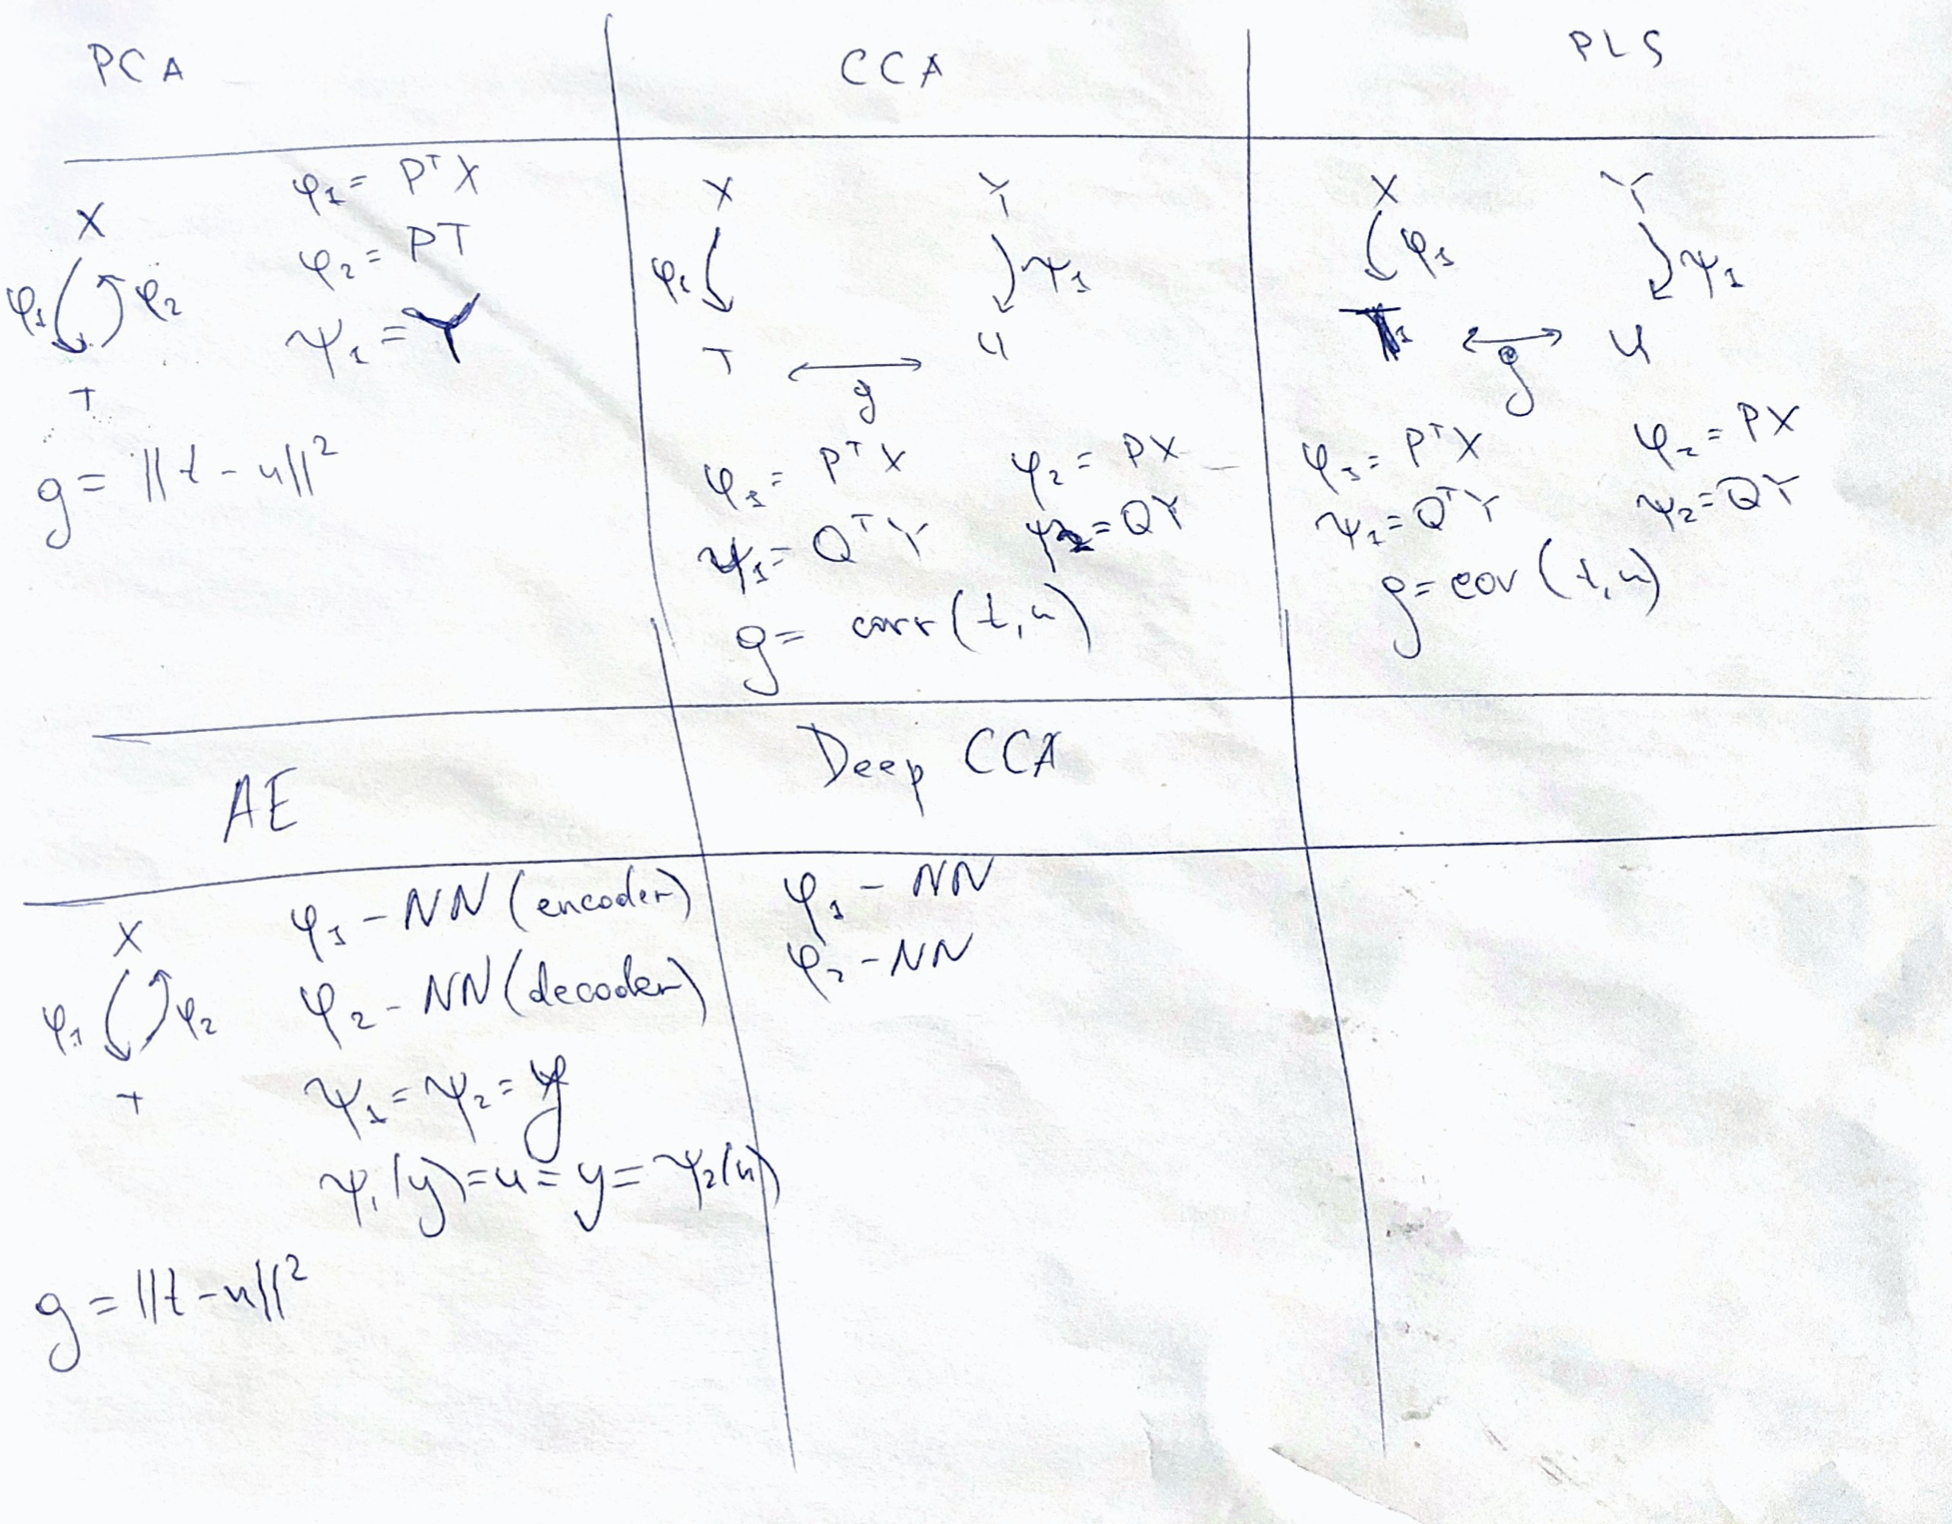
\includegraphics[width=\linewidth]{figs/ch1/Examples}
	\caption{Примеры алгоритмов, работающих по схеме \ref{ch1:eq:decoding_scheme}}
	\label{ch1:fig:PLSFigure}
\end{figure}

\subsection{Deep CCA}

Deep CCA~-- нелинейной модификация CCA. DCCA преобразует исходные данные с помощью многослойной нейронной сети таким образом, что результирующее представление становится согласованным. Предполагается, что есть $d$ слоев нейроной сети. 

Выходом первого слоя для экземпляра $\bx$ будет $\mathbf{h}_1 = s(\bW^{1}_{\bx}\bx + \bb^{1}_{\bx}) \in \mathbb{R}^{c_1}$, где $\bW_{\bx}^{1} \in \mathbb{R}^{c_1 \times m}$~-- матрица весов, $\bb_{x}^{1} \in \mathbb{R}^{c_1}$~-- вектор смещения, $s: \mathbb{R} \to \mathbb{R}$~-- нелинейная функция, которая действует покомпонентно. Далее выход первого слоя используется для вычисления выхода второго слоя $\mathbf{h}_{2} = s(\bW^{2}_{\bx}\mathbf{h}_{1} + \bb^{2}_{\bx}) \in \mathbb{R}^{c_2}$ и так далее до тех пор пока не будет найдено конечное представление $\varphi_e(\bx) = s(\bW^{d}_{\bx}\mathbf{h}_{d-1} + \bb^{d}_{\bx}) \in \mathbb{R}^{p}$. Аналогично находится представление для $\by$: $\psi_e(\by) = s(\bW^{d}_{\by}\mathbf{h}_{d-1} + \bb^{d}_{\by}) \in \mathbb{R}^{p}.$

Обозначим $\theta_{\bx}$, $\theta_{\by}$~-- параметры для функций кодирования, то есть матрицы весов и векторы смещений. Оптимальные параметры $\theta_{\bx}^{*}$, $\theta_{\by}^{*}$ находятся из задачи оптимизации:
\begin{equation}
(\theta_{\bx}^{*}, \theta_{\by}^{*}) = \argmax _{(\theta_{\bx}, \theta_{\by})} [g(\varphi_e(\bX; \theta_{\bx}), \psi_e(\bY; \theta_{2}))] = \argmax _{(\theta_{\bx}, \theta_{\by})} [corr(\varphi_e(\bX; \theta_{\bx}), \psi_e(\bY; \theta_{2}))].
\end{equation}

%%%%%%%%%%%%%%%%%%%%%%%%%%%%%%%%%%%%%%%%%%%%%%%%
\section{Вычислительный эксперимент}
%%%%%%%%%%%%%%%%%%%%%%%%%%%%%%%%%%%%%%%%%%%%%%%%

Временные ряды электроэнергии состоят из почасовых записей (52512 наблюдений). 
Строка матрицы~$\bX$~--– локальная история сигнала за одну неделю $n = 24 \times 7$. Строка матрицы~$\bY$~--- локальный прогноз потребления электроэнергии в следующие 24 часа $r = 24$. В этом случае матрицы~$\bX$ и~$\bY$ являются авторегрессионными матрицами.

Вычислительный эксперимент также проводился на данных электрокортикограмм (ECoG) из проекта NeuroTycho~\cite{shimoda2012decoding}.
Данные ECoG состоят из 32-канальных сигналов напряжения, снятых с головного мозга.
Цель состоит в предсказании по входному сигналу ECoG 3D позиции рук в последующие моменты времени.
Исходные сигналы напряжения преобразуются в пространственно-временное представление с помощью вейвлет-преобразования с материнским вейвлетом Морле.
Процедура извлечения признаков из исходных данных подробно описана в~\cite{chao2010long,eliseyev2016penalized}.
Описание исходного сигнала в каждый момент времени имеет размерность 32 (каналы) $\times $ 27 (частоты) = 864.
Каждый объект представляет собой локальный отрезок времени длительностью $\Delta t = 1s$. Временной шаг между объектами $\delta t = 0.05 s$.
Матрицы имеют размеры $\bX \in \bbR^{18900 \times 864}$ и $\bY \in \bbR^{18900 \times 3k}$, где $k$ - число отсчётов времени прогнозирования.
Данные разбиты на тренировочную и тестовую части в соотношении 0,67. 
Пример исходных сигналов мозга и соответствующей траектории руки показан на рисунке~\ref{ch2:fig:ecog_data}.

\begin{figure}
	\centering
	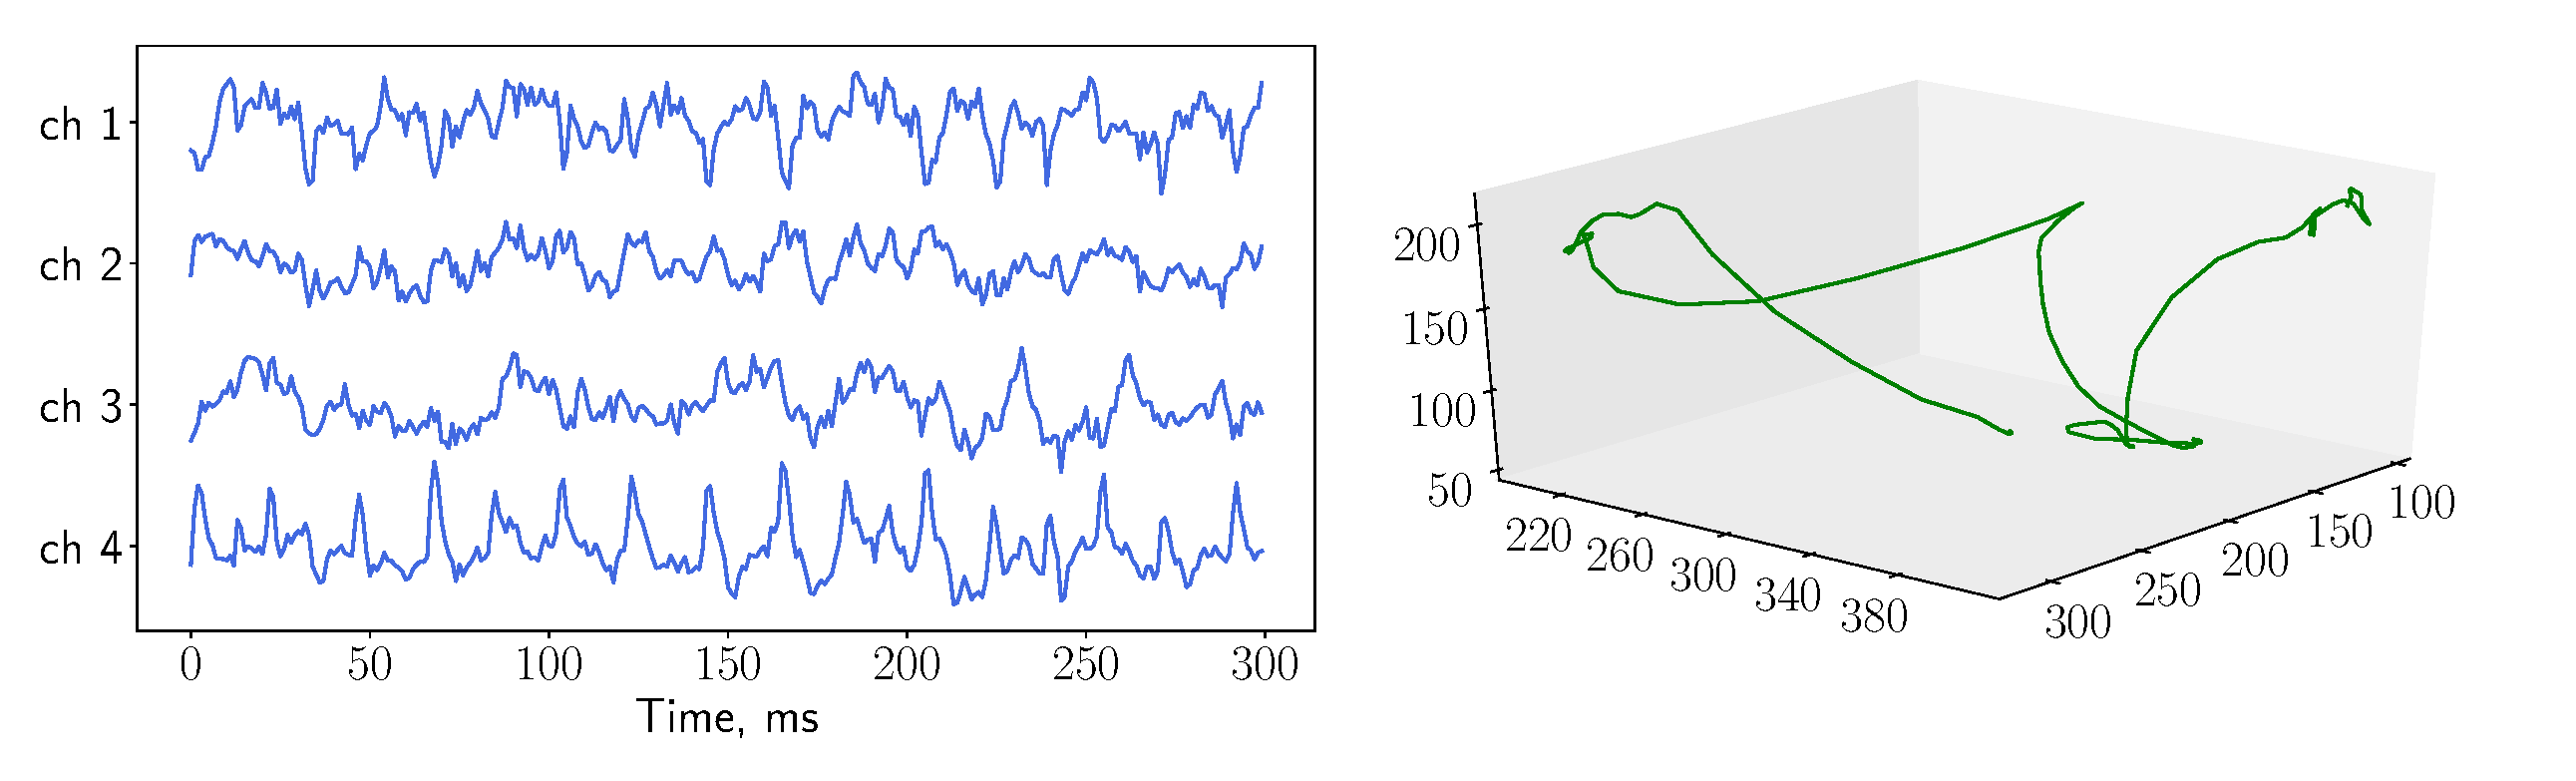
\includegraphics[width=\linewidth]{figs/ch2/ecog_data}
	\caption{Сигналы мозга (левый график) и 3D координаты руки (правый график)}
	\label{ch1:fig:ecog_data}
\end{figure}

Введём среднеквадратичную ошибку для некоторых матриц $\mathbf{A} = [a_{ij}]$ и $\mathbf{B} = [b_{ij}]$
\[
\text{MSE} (\mathbf{A}, \mathbf{B}) = \sum_{i,j} (a_{ij} - b_{ij})^2.
\]
Для оценивания качества аппроксимации вычисляется значение нормированной среднеквадратичной ошибки
\begin{equation}
\text{NMSE}(\bY,  \mathbf{\hat{Y}}) = \frac{\text{MSE} (\bY, \mathbf{\hat{Y}})}{\text{MSE} (\bY, \mathbf{\bar{Y}})},
\label{ch1:eq:nmse}
\end{equation}
где $\mathbf{\hat{Y}}$~--- прогноз модели, $\mathbf{\bar{Y}}$~--- константный прогноз средним значением по столбцам матрицы.

\subsection*{Данные потребления электроэнергии}

Для нахождения оптимальной размерности $l$ латентного пространства все данные потребления электроэнергии были разбиты на обучающую и валидационную части. 
Обучающая выборка состоит из $700$ объектов, валидационная из $370$. Зависимость нормированной квадратичной ошибки~\eqref{ch1:eq:nmse} от размерности $l$ латентного пространства представлена на Рис.~\ref{ch1:fig:energy_n_comp}. 
Сначала ошибка резко падает при увеличении размерности скрытого пространства, а затем стабилизируется.

\begin{figure}[ht]
	\centering
	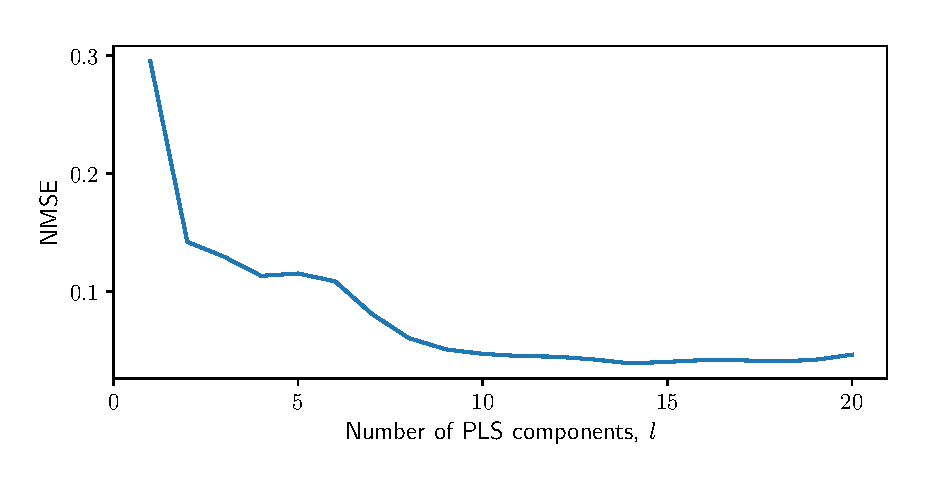
\includegraphics[width=0.75\linewidth]{figs/ch1/energy_n_comp}
	\caption{Прогноз потребления электроэнергии алгоритмом PLS при размерности латентного пространства $l$=14}
	\label{ch1:fig:energy_n_comp}
\end{figure}

Минимальная ошибка наблюдается при $l=14$. 
Построим прогноз потребления электроэнергии при данном $l$. 
Результат аппроксимации изображен на Рис.~\ref{ch1:fig:energy_prediction}. Алгоритм PLS восстановил авторегрессионную зависимость и обнаружил дневную сезонность.

\begin{figure}[ht]
	\centering
	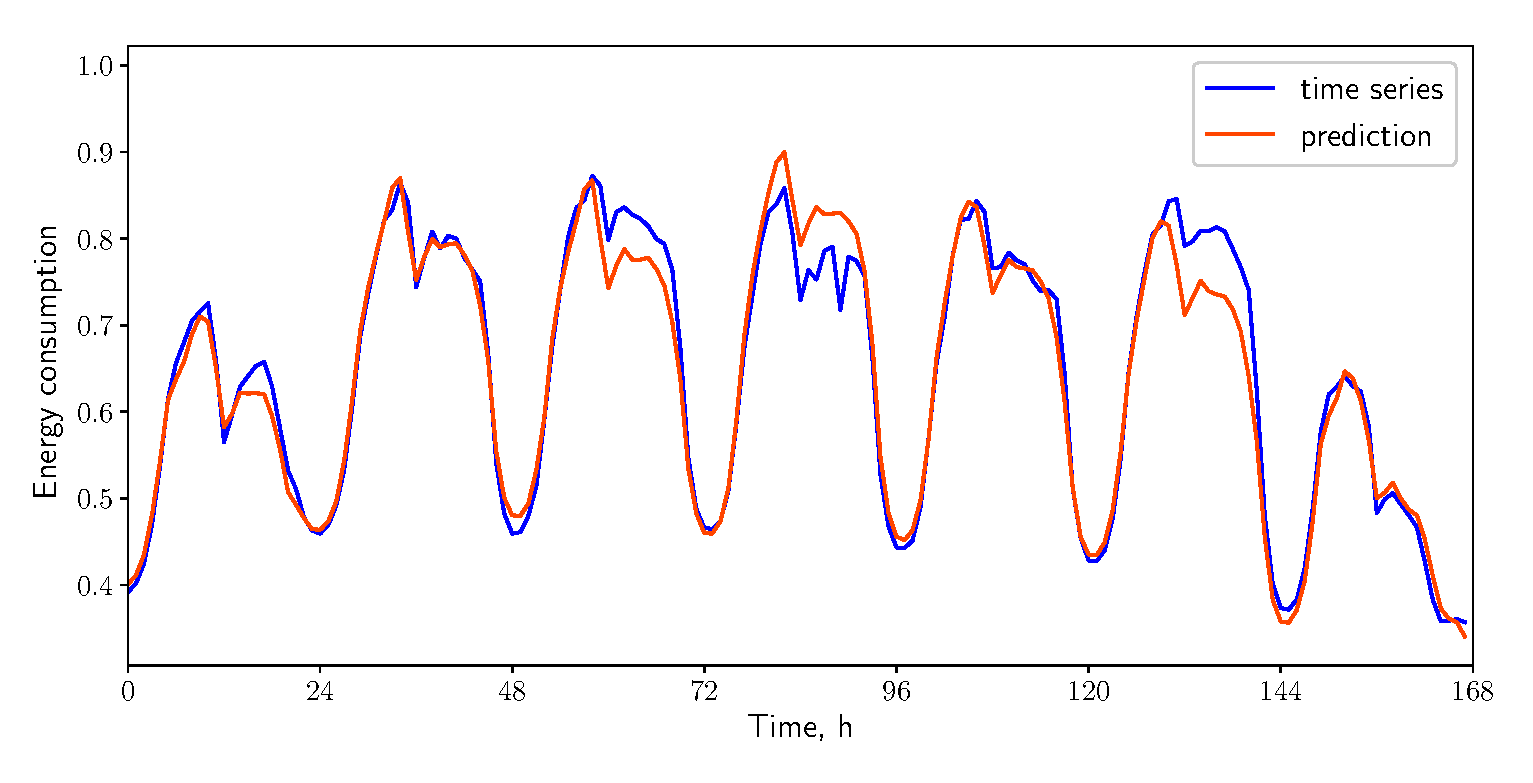
\includegraphics[width=0.95\textwidth]{figs/ch1/energy_prediction}
	\caption{Зависимость ошибки от размерности латентного пространства для данных потребления электроэнергии}
	\label{ch1:fig:energy_prediction}
\end{figure}

\subsection*{Данные электрокортикограммы}

На Рис.~\ref{ch1:fig:ecog_n_comp} представлена зависимость нормированной квадратичной ошибки~\eqref{ch1:eq:nmse} от размерности латентного пространства. Ошибка аппроксимации меняется незначительно при $l > 5$.
Таким образом совместное описание пространственно-временного спектрального представления объектов и пространственного положения руки может быть представлено вектором размерности $l \ll n$.
Зафиксируем $l = 5$. 
Пример аппроксимации положения руки изображен на Рис.~\ref{ch1:fig:ecog_prediction}. 
Сплошными линиями изображены истинные координаты руки по всем осям, пунктирными линиями показана аппроксимация методом PLS.
 
\begin{figure}[ht]
	\centering
	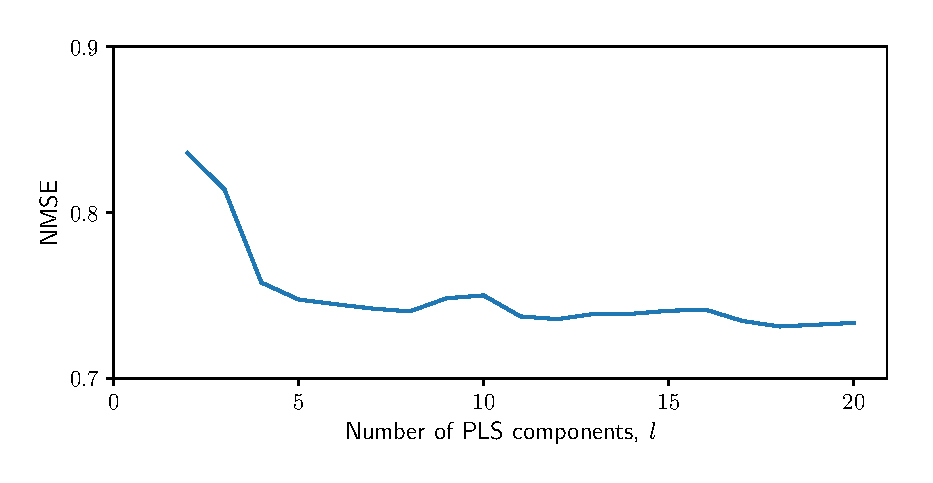
\includegraphics[width=0.75\linewidth]{figs/ch1/ecog_n_comp}	
	\caption{Зависимость ошибки от размерности латентного пространства для данных ECoG}
	\label{ch1:fig:ecog_n_comp}
\end{figure}

\begin{figure}[ht]
	\centering
	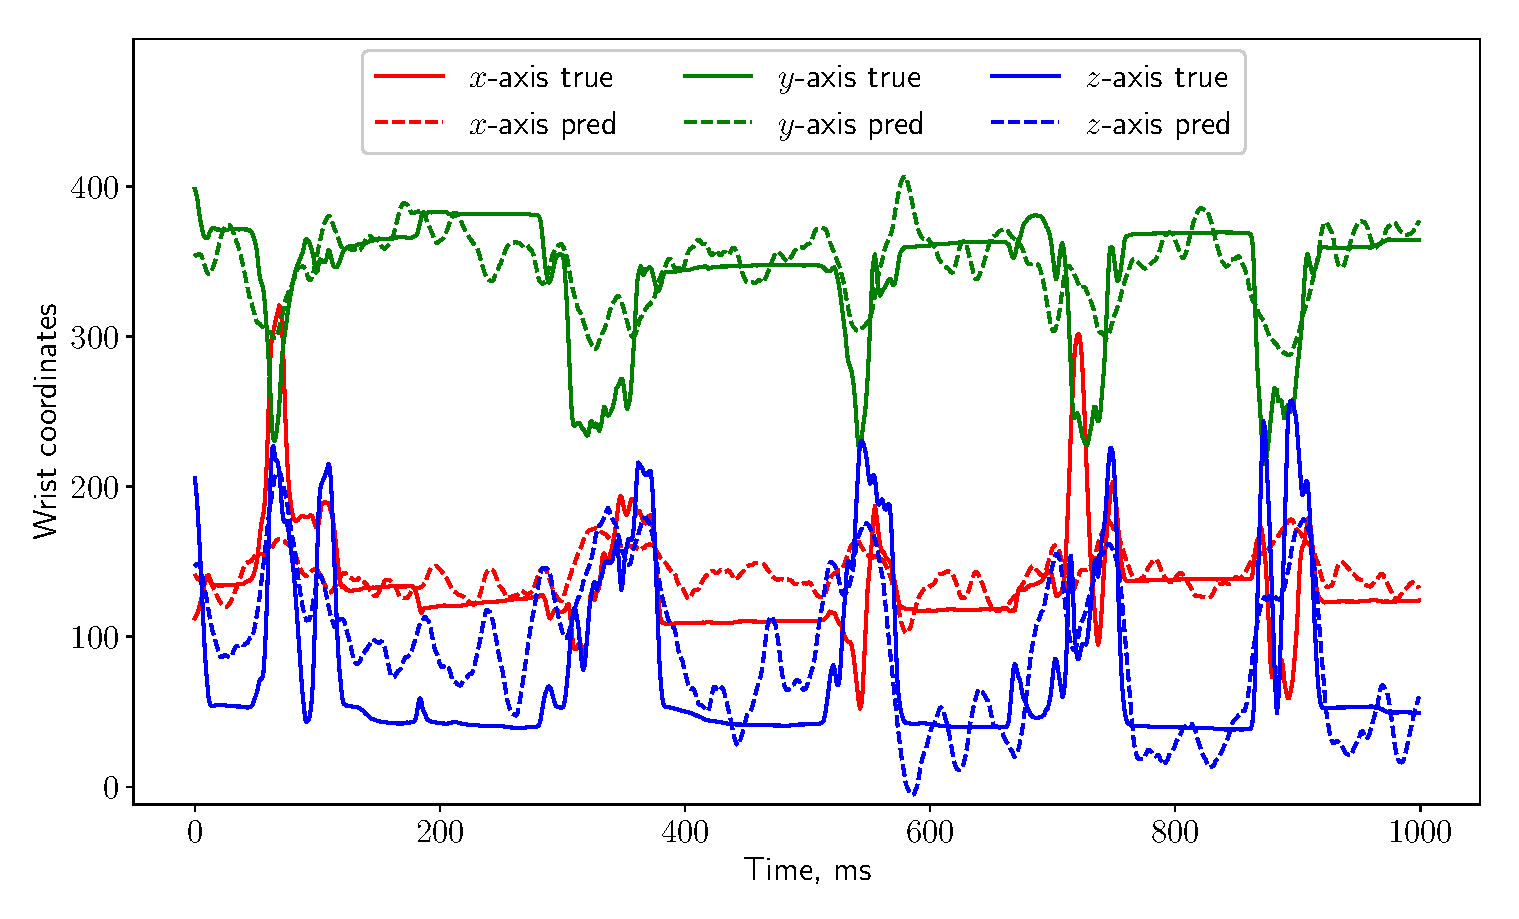
\includegraphics[width=\textwidth]{figs/ch1/ecog_prediction}
	\caption{Прогноз движения руки по данным ECoG алгоритмом PLS при размерности латентного пространства $l=5$}
	\label{ch1:fig:ecog_prediction}
\end{figure}

